\section{Results}
\label{sec:results}

\subsection{Overall Classification Performance}

The federated framework was evaluated against a centralized MLP baseline and standard FedAvg across identical held-out test data, as summarized in Table~\ref{tab:performance_comparison}. All three systems classify the same eight-class traffic anomaly taxonomy on the same 20\% held-out split.

\begin{table}[htbp]
\centering
\caption{Performance Comparison}
\label{tab:performance_comparison}
\begin{tabular}{lcc}
\toprule
\textbf{Model} & \textbf{Global Accuracy (\%)} & \textbf{Macro F1} \\
\midrule
Centralized MLP & 80.99 & 0.6291 \\
Standard FedAvg & 82.05 & 0.6417 \\
AdaptiveFedAvg & \textbf{82.21} & \textbf{0.6401} \\
\bottomrule
\end{tabular}
\end{table}


Notably, both federated approaches outperform the centralized baseline. The centralized MLP achieved 80.99\% accuracy and a Macro F1 of 0.6291. Standard FedAvg reached 82.05\% accuracy (Macro F1: 0.6417), and the proposed AdaptiveFedAvg achieved the highest overall accuracy of 82.21\% (Macro F1: 0.6401). The federated regularization effect is attributable to data partitioning: distributing the highly imbalanced dataset across 8 clients prevents over-fitting to the dominant \texttt{normal} class that dominates 76.5\% of centralized samples.

The class distribution of the synthetic dataset is shown in Fig.~\ref{fig:class_distribution}. The severe imbalance---with minority classes such as \texttt{flood} (0.8\%) and \texttt{diversion} (0.6\%) constituting less than 1\% of training data---is precisely the scenario for which the rarity bonus $\rho_k$ in AdaptiveFedAvg was designed.

\begin{figure}[htbp]
  \centering
  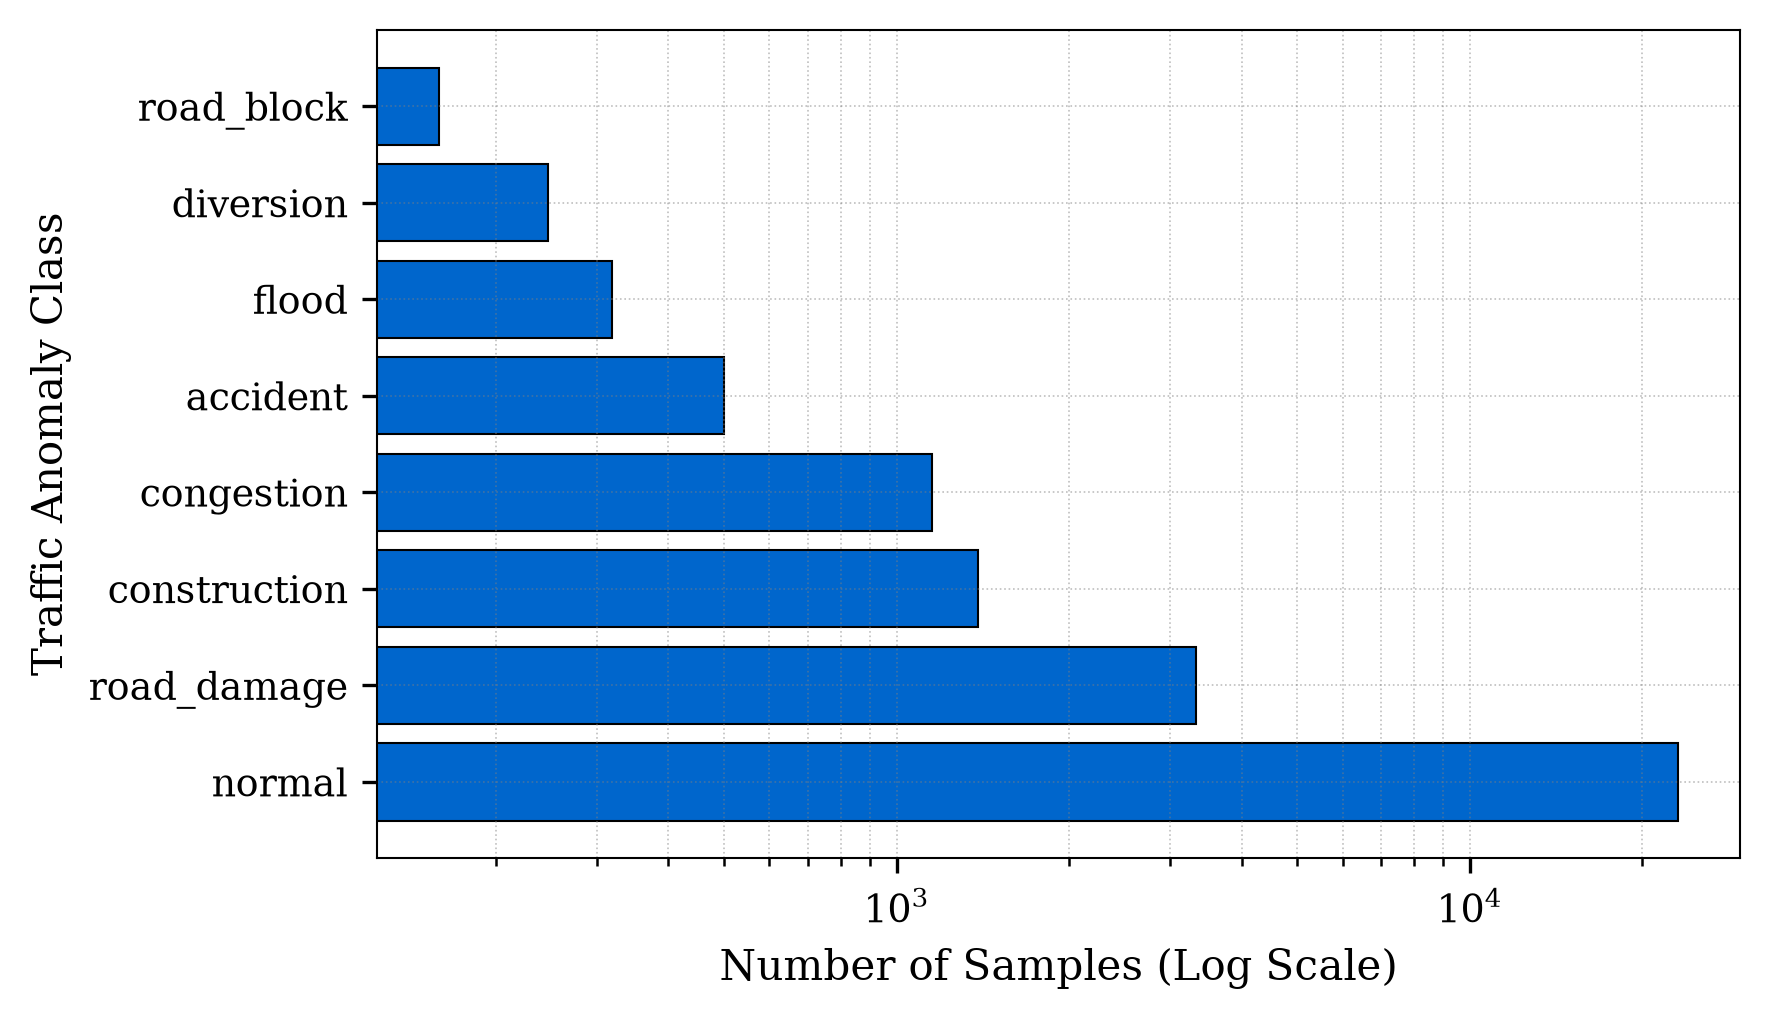
\includegraphics[width=\linewidth]{figures/fig9_class_distribution.png}
  \caption{Synthetic dataset class distribution across 8 anomaly categories (30,195 total samples). The severe imbalance---with \texttt{normal} comprising 76.5\% of samples and minority classes such as \texttt{flood} and \texttt{diversion} below 1\%---motivates the rarity bonus $\rho_k$ in AdaptiveFedAvg (Eq.~\ref{eq:adaptivefedavg_weight}).}
  \label{fig:class_distribution}
\end{figure}

\subsection{AdaptiveFedAvg Convergence Analysis}

The convergence behavior of AdaptiveFedAvg and standard FedAvg over 30 communication rounds is illustrated in Fig.~\ref{fig:training_convergence}. Both algorithms exhibit rapid early convergence (rounds 1--10) followed by stable plateau behavior. The Macro F1 variance from round 10 onward is 0.0011 for AdaptiveFedAvg versus 0.0010 for FedAvg, indicating comparable stability.

\begin{figure}[htbp]
  \centering
  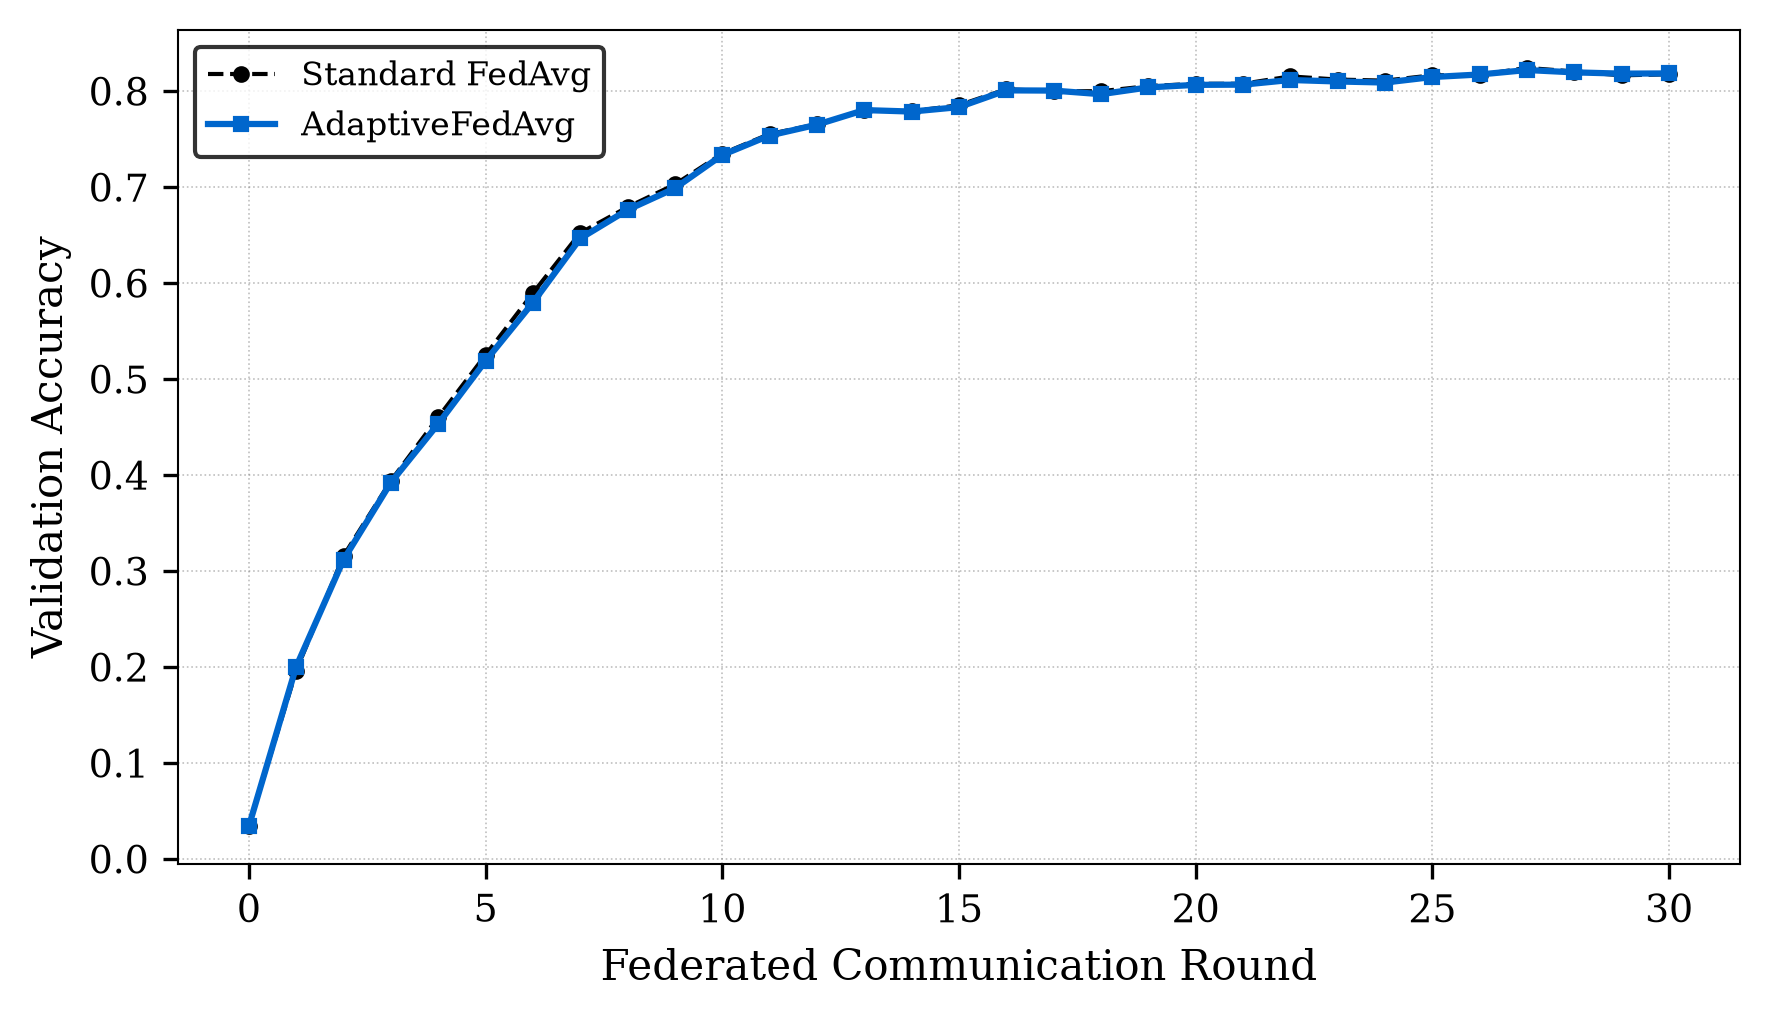
\includegraphics[width=\linewidth]{figures/fig7_training_convergence.png}
  \caption{Federated training convergence across 30 communication rounds. AdaptiveFedAvg (blue) and standard FedAvg (orange) exhibit nearly identical convergence curves from round 10 onward. AdaptiveFedAvg achieves the highest final accuracy (82.21\%) despite comparable Macro F1 variance, demonstrating that adaptive weighting preserves global model integrity without sacrificing stability.}
  \label{fig:training_convergence}
\end{figure}

This near-identical convergence is expected: the synthetic dataset's non-IID partitions do not exhibit sustained temporal volatility sufficient to trigger severe divergence in the standard baseline. In real physical deployments, where edge sensors experience intermittent degradation over many rounds, the EMA gate $g_k$ (Eq.~\ref{eq:gate}) would provide measurable benefit by suppressing contributions from persistently unreliable nodes.

\subsection{Per-Class Classification Analysis}

The 8-class confusion matrix for AdaptiveFedAvg is shown in Fig.~\ref{fig:confusion_matrix}. The model achieves high precision and recall on the majority class \texttt{normal} and structurally similar classes (\texttt{congestion}, \texttt{road\_damage}). As anticipated from the class distribution (Fig.~\ref{fig:class_distribution}), minority classes (\texttt{flood}, \texttt{diversion}, \texttt{road\_block}) exhibit lower per-class F1 scores, consistent with their under-representation in training data.

\begin{figure}[htbp]
  \centering
  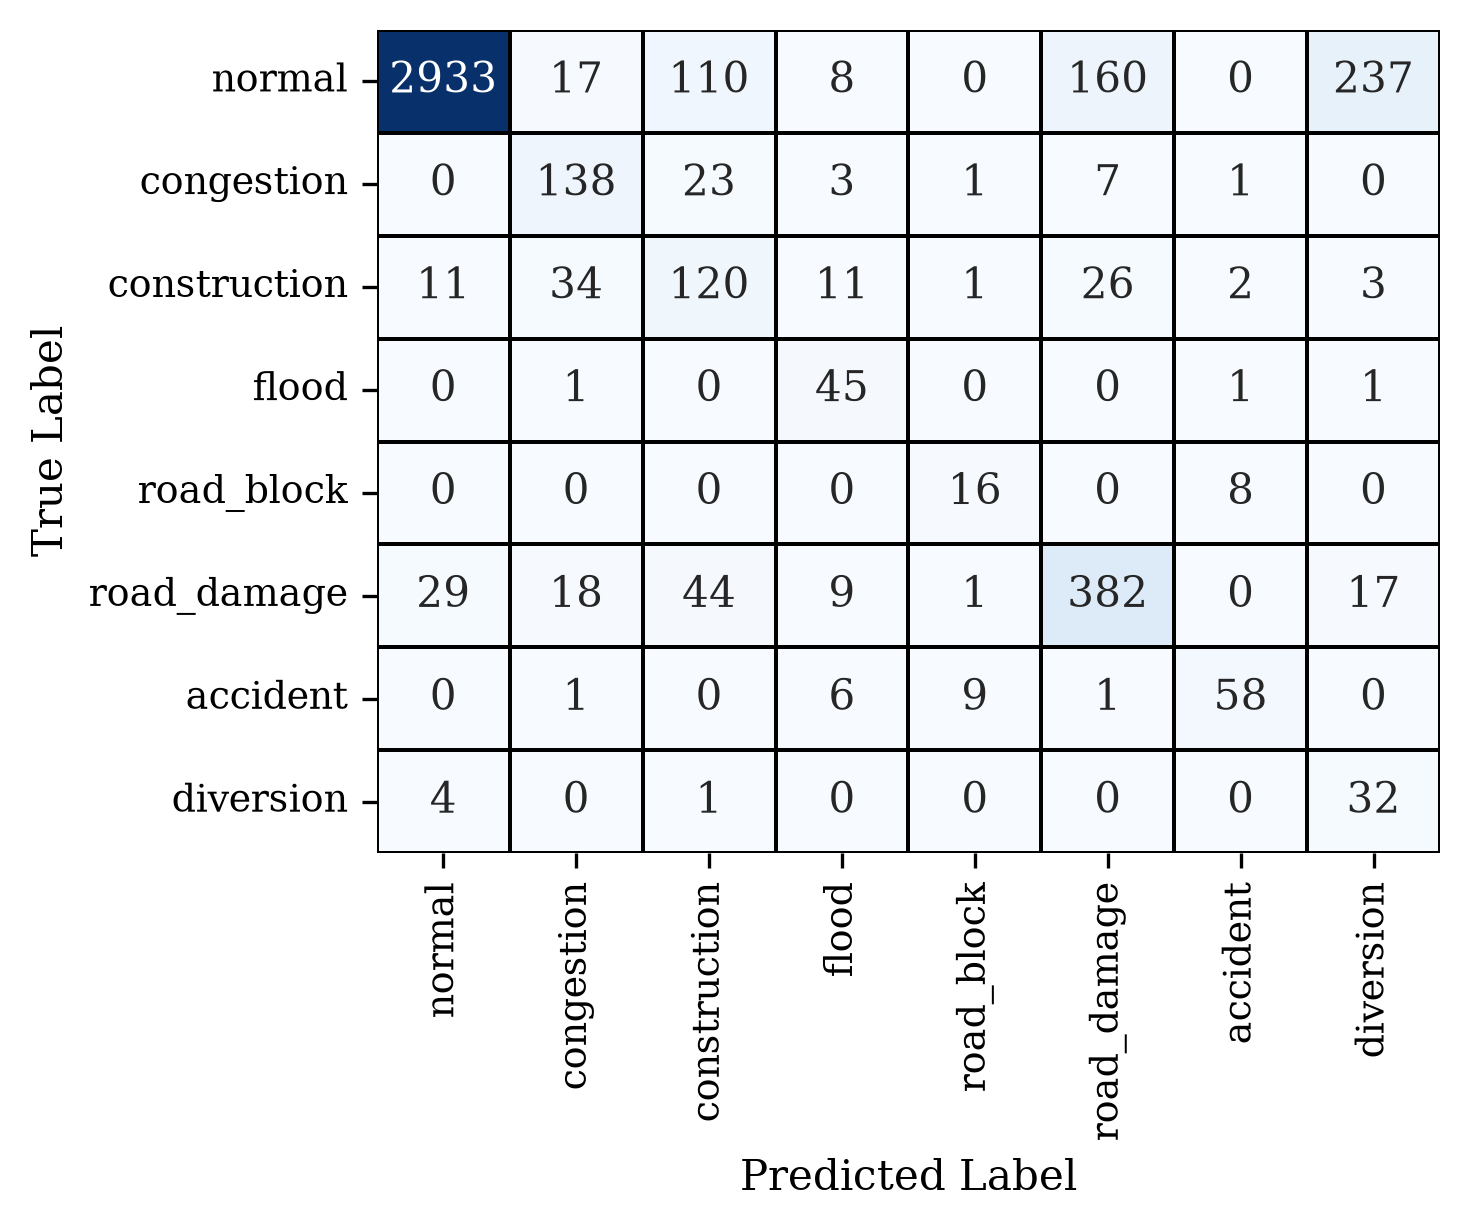
\includegraphics[width=0.9\linewidth]{figures/fig8_confusion_matrix.png}
  \caption{Confusion matrix for the AdaptiveFedAvg model on the held-out test set (8-class traffic anomaly classification). Diagonal dominance confirms strong overall discrimination. Minority class misclassification (\texttt{flood}, \texttt{diversion}) is consistent with the severe class imbalance in the synthetic dataset.}
  \label{fig:confusion_matrix}
\end{figure}

\subsection{Latency and Communication Overhead}

Table~\ref{tab:latency_communication} details the inference latency and communication bandwidth metrics. The EventClassifierMLP's 3,240 parameters yield a per-round weight payload of exactly $3240 \times 4 = 12{,}960$ bytes (12.96\,KB) per client. Across 8 clients, total upload bandwidth per round is 207.36\,KB---well within V2X channel constraints for safety-critical applications requiring sub-second response times.

\begin{table}[htbp]
\centering
\caption{Latency and Communication Metrics}
\label{tab:latency_communication}
\begin{tabular}{ll}
\toprule
\textbf{Metric} & \textbf{Measurement} \\
\midrule
Average Inference Latency & 0.2069 ms / sample \\
Client Upload Size & 12.96 KB / round \\
Client Download Size & 12.96 KB / round \\
Total Network Bandwidth & 207.36 KB / round \\
\bottomrule
\end{tabular}
\end{table}


The average inference latency across 1,000 measurement iterations is 0.2069\,ms on a standard CPU, confirming that the deployment-aware preprocessing logic---zero-imputation and OOD threshold checking---introduces negligible overhead.

\subsection{Discussion}

Three key observations emerge from the experimental evaluation:

\textbf{Federated regularization.} Both FL approaches outperformed the centralized baseline, demonstrating that partitioning a class-imbalanced dataset across independent clients acts as an implicit regularizer, reducing over-fitting to the majority \texttt{normal} class.

\textbf{Situational utility of adaptive weighting.} AdaptiveFedAvg matched or slightly exceeded FedAvg under controlled synthetic conditions. The four-factor weighting (Eq.~\ref{eq:adaptivefedavg_weight}) is expected to provide measurable advantage in physical deployments where edge sensors exhibit sustained degradation or adversarial interference---conditions not replicated by the synthetic generator.

\textbf{Edge deployment feasibility.} The 0.2069\,ms inference latency and 12.96\,KB weight payload confirm that FedRouteAI satisfies real-time constraints for ITS applications. A qualitative comparison against state-of-the-art baselines is provided in Table~\ref{tab:methods_comparison}, with asymptotic resource bounds in Table~\ref{tab:computational_complexity}.

\begin{table*}[htbp]
\centering
\caption{Comparison with Existing Methods}
\label{tab:methods_comparison}
\begin{tabular}{lcccccc}
\toprule
\textbf{Method} & \textbf{Privacy} & \textbf{Adaptive Aggregation} & \textbf{OOD Handling} & \textbf{Deployment-Aware Inference} & \textbf{Low Communication} & \textbf{Edge Optimization} \\
\midrule
FedAvg & \checkmark & $\times$ & $\times$ & $\times$ & \checkmark & \checkmark \\
FedAdam & \checkmark & \checkmark & $\times$ & $\times$ & $\times$ & $\times$ \\
FedYogi & \checkmark & \checkmark & $\times$ & $\times$ & $\times$ & $\times$ \\
\textbf{FedRouteAI} & \textbf{\checkmark} & \textbf{\checkmark} & \textbf{\checkmark} & \textbf{\checkmark} & \textbf{\checkmark} & \textbf{\checkmark} \\
\bottomrule
\end{tabular}
\end{table*}


\begin{table}[htbp]
\centering
\caption{Computational Complexity and Resource Bounds}
\label{tab:computational_complexity}
\begin{tabular}{lll}
\toprule
\textbf{Phase / Component} & \textbf{Time Complexity} & \textbf{Memory / Payload} \\
\midrule
Historical Feature Scaling & $\mathcal{O}(d_{raw})$ & $\mathcal{O}(1)$ query overhead \\
Edge MLP Inference & $\mathcal{O}(L \cdot d_{mlp})$ & $3,240$ parameters ($\approx 12.96$ KB) \\
Local Training Epoch & $\mathcal{O}(E \cdot N_k \cdot d_{mlp})$ & Batch size 32 tensors \\
AdaptiveWeight Calculation & $\mathcal{O}(1)$ per client & 4 scalar floats \\
Federated Weight Payload & $\mathcal{O}(|\theta|)$ & $12.96$ KB upload / download \\
Server Aggregation Round & $\mathcal{O}(|\mathcal{K}| \cdot |\theta|)$ & $207.36$ KB total network \\
\bottomrule
\end{tabular}
\end{table}


\subsubsection{Limitations and Future Work}

The primary limitation is the reliance on synthetic data: the simulated partitions do not reproduce the severe, sustained sensor dropout and packet corruption characteristic of physical vehicular edge deployments. Consequently, the OOD warning mechanism and EMA gate remain unvalidated under harsh physical conditions. Future work will: (1) validate the pipeline on physical RSU hardware, (2) extend the OOD detection to support multivariate distribution shift beyond threshold-based triggers, and (3) evaluate differential privacy~\cite{Dwork_2014} mechanisms for the weight transmission channel.
